\documentclass{ctexart}
\usepackage[T1]{fontenc}
\usepackage[a4paper,top=1.5cm,bottom=1.5cm,left=2cm,right=2cm,marginparwidth=1.75cm]{geometry}
\usepackage{mathtools}
\usepackage{tikz}
\usepackage{booktabs}
\usepackage{caption}
\usepackage{outlines}
\usepackage{graphicx}
\usepackage{amsthm}
\usepackage{tabu}
\usepackage{minted}
\usepackage[colorlinks=false, allcolors=blue]{hyperref}
\usepackage{cleveref}
% \usepackage{soul}
% \usepackage{sout}
\usepackage{ulem}
\renewcommand{\tableautorefname}{表}
\DeclarePairedDelimiter{\set}{\{}{\}}
\DeclarePairedDelimiter{\paren}{(}{)}
\graphicspath{ {./images/} }
\newcommand*{\fullref}[1]{
\ifthenelse{\equal{\thepage}{\getpagerefnumber{#1}}}
  {
    \hyperref[{#1}]{\Cref*{#1} \nameref*{#1}}
  }
  {% false case
    \hyperref[{#1}]{第 \pageref*{#1} 页 \Cref*{#1} \nameref*{#1}}
  }
}

\title{操作系统第八次作业}
\author{卢雨轩 19071125}
% \date{\today}
\ctexset{
    section = {
        titleformat = \raggedright,
        name = {,},
        number = \chinese{section}、
    },
    paragraph = {
        runin = false
    },
    today = small,
    figurename = 图,
    contentsname = 目录,
    tablename = 表,
}

\begin{document}

\maketitle

\begin{outline}[enumerate]
    \1 为什么文件分配的位图必须保存在大容量存储器中,而不是主存中?

        因为主存在重启后内容会全部丢失。

    \1 假设要为一个文件换一个名字。一种选择是使用操作系统提供的RENAME方法,另一种方法是:把文件复制为新文件,然后删除原来的文件以实现重命名。请问,这两种方法在实现上有什么不同? 

        前者实现上,是修改指向 FCB 的指针的名称,以及FCB中文件名。后者的实现是创建一个新的FCB,复制数据块,最后删除旧的 FCB 和数据块。

    \1 请解释使用索引节点有什么好处

        节省启动磁盘的次数,提高运行效率。
    \1 在UNIX中open系统调用绝对需要么?如果没有会产生什么结果。

        需要。首先,操作系统可以记录进程所拥有的文件资源,并在进程终止时回收。如果没有,直接把文件名传入write调用的话,可能会出现资源泄漏(如进程没有正确关闭文件,导致仍有内容在文件的输入输出缓存中)。

    \begin{minipage}[b]{0.7\textwidth}
        \1 UNIX系统中有关盘块的分配与释放是借助超级块中的栈来进行的。假如某个时刻系统状况如下图所示,若此时某个进程要删除文件A,并归还它所占用的盘块220,110,645,549,176。请说明过程,并给出删除完毕后有关数据及表目的更改情况。

        首先放入220,110,645。此时,共有100个空闲块,于是将栈内内容写入549,栈中只剩下549。之后176入栈。
        
        \1 有一个文件系统,根目录常驻内存,如图所示。目录文件采用链接结构,每个目录下最多存放60个文件或目录(称为下级文件)。每个磁盘块最多可存放10个文件目录项:如果下级文件是目录文件,则上级目录项指向该目录文件的第一块地址。假设目录结构中文件或子目录按自左向右的次序排列,…表示尚有其他文件或子目录。 
    \end{minipage}%
    \begin{minipage}[t]{0.3\textwidth}
        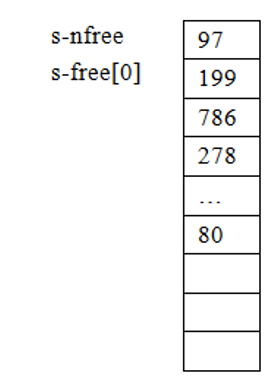
\includegraphics[width=\linewidth]{8-5.png}
    \end{minipage}
        \2 普通文件采用UNIX三级索引结构,每个索引节点可以保存10个直接地址,并假设每个磁盘块可以保存128个磁盘地址。主索引表放在目录项中,若要读/A/D/G/I/K的第16520块,最少启动硬盘几次,最多几次?

            目录访问:A已经在内存里。访问DJIK分别需要1,1-6,1-6,1-6次,最少4次,最多19次。
            
            得到K的inode后,需要读出K的FCB,一次。

            之后需要读出K的二级索引,2次。

            最后读内容,1次。

            所以,8次到23次。
        
            \sout{最少: $\underbrace{1 \times 2}_{A, D} + \underbrace{3 \times 1}_{G,I,K} + 3 = 8$次}

            \sout{最多: $\underbrace{1 \times 2}_{A, D} + \underbrace{3 \times 6}_{G,I,K} + 3 = 23$次。
            }

        \2 若普通文件采用顺序结构,若要读/A/D/G/I/K的第1185块,最少启动硬盘几次,最多几次?

            最少: $5 + 1 = 6$次

            最多: $20 + 1 = 21$次。
    
    \1 考虑一个索引节点所表示的UNIX文件的组织。假设有12个直接块指针,在每个索引节点中有一个单重、双重和三重间接指针。此外,假设系统块大小和磁盘扇区大小都是8K,如果磁盘块指针是32位,其中8位表示物理磁盘,24位表示物理块,那么
    \2 该系统支持的最大文件大小是多少?

        \sout{$8000 \times 12 + 8000 / 32 \times 8000 + 8000 / 32 \times 8000 / 32 \times 8000 + 8000 / 32 \times 8000 / 32 \times 8000 / 32 \times 8000 = 125,502,096,000 \approx 125.5$GB}

        $8192 \times 12 + 8192 / 4 \times 8192 + 8192 / 4 \times 8192 / 4 \times 8192 + 8192 / 4 \times 8192 / 4 \times 8192 / 4 \times 8192 = 96k + 16M + 32G + 64T$
    \2 该系统支持的最大文件分区是多少?

        \sout{$2^{24} \times 8000 = 134,217,728,000 \approx 134GB$}

        $2^{24} \times 8192 = 128G$
    \2 假设主存中除了文件索引节点外没有其他信息,访问在位置12423956中的字节需要多少磁盘访问?

        \sout{4次。}
        
        2次。

\end{outline}

\end{document}
